\section{Neutron Irradiation}
\label{sec:irradiation}

\subsection{Rhode Island Neutron Irradiation Facility}
\label{subsec:RINSC}
RINSC (Rhode Island Nuclear Science Center) is a 2 MW, light water cooled, pool type reactor in Narragansett, Rhode Island, USA.
The core consists of fuel assemblies reflected with a combination of graphite and beryllium.
The fuel is plate type U3Si2 cladded with aluminum enriched to less than 20% Uranium-235.
At RINSC there are three (six?) different ways to irradiate materials: beamports (pipes that run from the work area to the reactor core), rabbit system (pneumatic system that ferries plastic sample bottles to the reactor core), and InCore tubes (small samples are placed into a tube and lowered into an empty basket next to the fuel elements). 
The beamports can accomodate samples of up to 7.75" x 3' [diameter by length], the rabbit system can accept sampes 1.125" x 6.25", and the InCore system can irradiate objects 1.25" x 9". 
Of the irradiation methods available, only the beamports are large enough to accomodate the silicon sensors for this project.
\begin{itemize}
    \item Fig 1 - image(s) of reactor core, beamport (see figure~\ref{fig:RINSC_Facility})
    what other details are useful here?
    Is it better to omit the sample irradiation options that are not being used?
    \item Fig 2 - puck design/layout, real pucks (see figure~\ref{fig:Pucks_Arrayed})
    \item Fig 3 - puck layout, packing (see figure~\ref{fig:Puck_Packing}), how much detail about packing materials? (see figure~\ref{fig:Cylinder_Details})
    \item Fig 4 - other hardware, cylinder, temp monitoring setup (see figure~\ref{fig:Temperature_Monitoring_Setup})
    Keithley 2400 for temperature readout (along with 20-channel input board), RTDs instrumented with ~20' of radiation-resistant wire (McMaster #?), laptop with GPIB connection to keithely, and custom LabVIEW code for readout.
    \item Fig 5 - schemaitc of experimental setup? Is this needed?
    \item describe sample removal/storage after irradiation
    \item describe fluence measurement setup/procedure at Brown? 
\end{itemize}

  \begin{figure}[!hbt]
  \begin{center}
    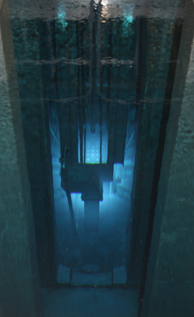
\includegraphics[width=0.25\textwidth]{figures/RINSC_Reactor_Core}
    \includegraphics[width=0.40\textwidth]{figures/Beamport_View}
    \caption{On the left is an image of the reactor core at RINSC, and on the right is a view down the beamport used for these irradiation studies.}
    \label{fig:RINSC_Facility}
  \end{center}
\end{figure}

\begin{figure}[!hbt]
  \begin{center}
    \includegraphics[width=0.70\textwidth]{figures/Hockey_Pucks_Arrayed}
    \caption{Sample containers ('hockey pucks') for sensors to be irradiated in the beamport at RINSC. The materials are wood (oak), acrylic, and PEEK.}
    \label{fig:Pucks_Arrayed}
  \end{center}
\end{figure}

\begin{figure}[!hbt]
  \begin{center}
    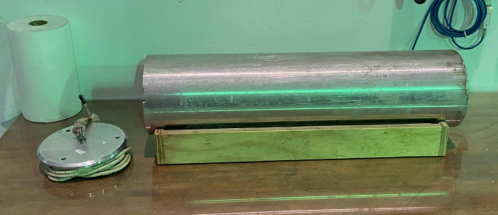
\includegraphics[width=0.70\textwidth]{figures/Cylinder_Side_View}
    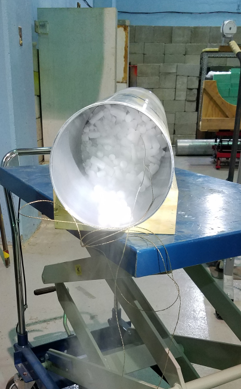
\includegraphics[width=0.70\textwidth]{figures/Cylinder_With_Dry_Ice}
    \caption{Left: aluminum cylinder used to transport hockey puck containers into the beamport. Right: cylinder containing a sample puck along with dry ice for cooling.}
    \label{fig:Cylinder_Details}
  \end{center}
\end{figure}

  \begin{figure}[!hbt]
  \begin{center}
    \includegraphics[width=0.20\textwidth]{figures/Hockey_Puck_Base_Instrumented}  
    \includegraphics[width=0.25\textwidth]{figures/Hockey_Puck_Sensor_Fit}
    \includegraphics[width=0.25\textwidth]{figures/Hockey_Puck_Kapton_Layer}
    \includegraphics[width=0.20\textwidth]{figures/Hockey_Puck_Lid_Instrumented}    
    \caption{Four views of sensor container packing: the base instrumented with fluence monitoring diodes, the fit of a sensor in the hockey puck, the protection of the sensor with layers of kapton foil, and the lid of the hockey puck instrumented with monitoring devices.}
    \label{fig:Puck_Packing}
  \end{center}
\end{figure}

\begin{figure}[!hbt]
  \begin{center}
    \includegraphics[width=0.80\textwidth]{figures/Temperature_Monitoring_Setup}
    \caption{Temperature monitoring setup for use during beamport irradiations at RINSC.}
    \label{fig:Temperature_Monitoring_Setup}
  \end{center}
\end{figure}

\subsection{List of Neutron-Irradiated Sensors}
\begin{itemize}
  \item full table of sensors irradiated in first campaign. Do we want to include sensors irradiated prior to the main campaign? On the order of 10 or so sensors maximum.
\end{itemize}

\begin{figure}[!hbt]
  \begin{center}
    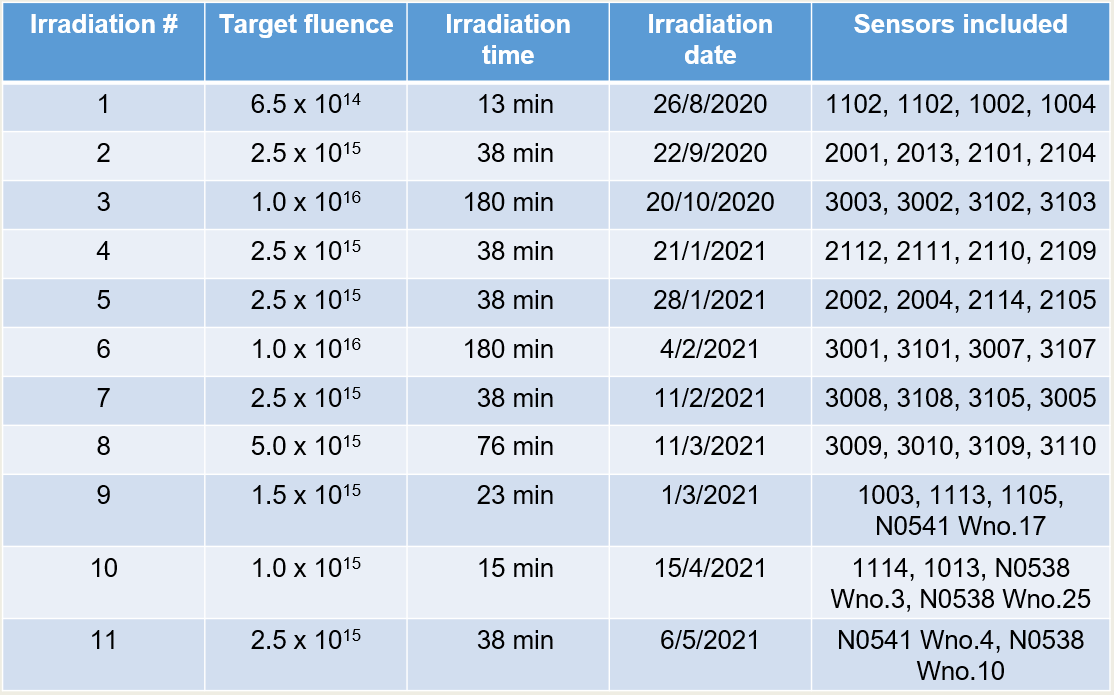
\includegraphics[width=0.90\textwidth]{figures/Completed_Irradiation_Schedule_at_RINSC}
    \caption{Completed irradiation schedule for all sensors irradiated in this campaign.}
    \label{fig:Irradiation_Schedule}
  \end{center}
\end{figure}

\label{subsec:sensors_irradiation}
